\chapter{Anonymisation des images DICOM}

Pour anonymiser les données, j'utilise le programme "Santé Dicom Editor". Il suffit d'ouvrir le dossier contenant les images et aller dans l'onglet Edit $\rightarrow$ Anonymise current file/series. Il existe des fonctions Matlab pour faire le même travail mais certains champs sensibles étaient malgré tous intacts. Voir \textit{http://www.santesoft.com/win/sante\_ dicom\_ editor/sante\_ dicom\_ editor.html}.

\begin{figure}[H]
\centering
    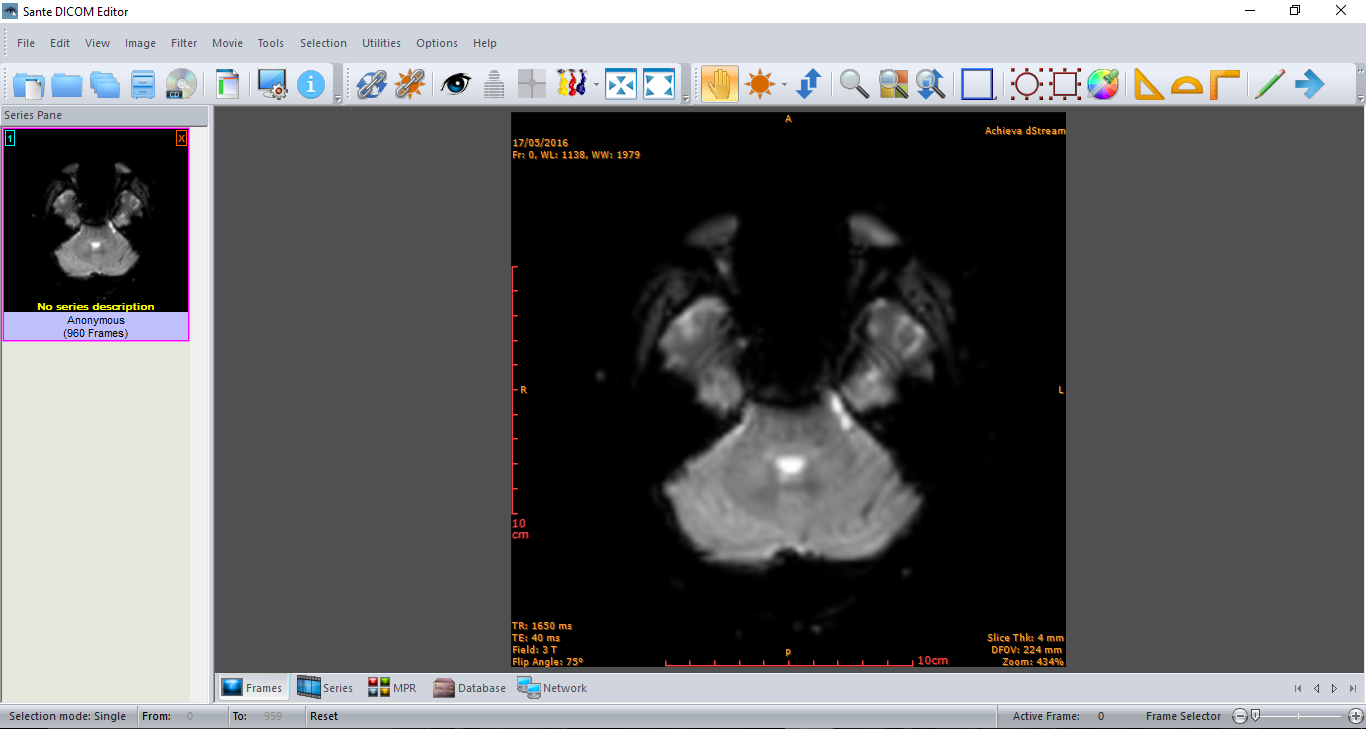
\includegraphics[scale=0.35,angle=90]{Images/AnonExe.png}
    \caption{Programme pour l'anonymisation des données.}
    \label{fig:AnonExe}
\end{figure}

\chapter{Visualisation des données en 3D et 4D}

Un gros problème lorsque nous recevons les images Dicom est que nous ne pouvons voir de façon très claire la localisation de la tumeur. J'ai donc réutilisé et modifié des codes Matlab disponibles sur internet afin d'avoir une représentation 3D et 4D. Ils sont disponibles sur les liens suivant:

\medskip

\textit{http://fr.mathworks.com/matlabcentral/fileexchange/41465-4d-volume-visualization}

\textit{http://www.mathworks.com/matlabcentral/fileexchange/37268-3d-volume-visualization}



\begin{figure}[H]
\centering
    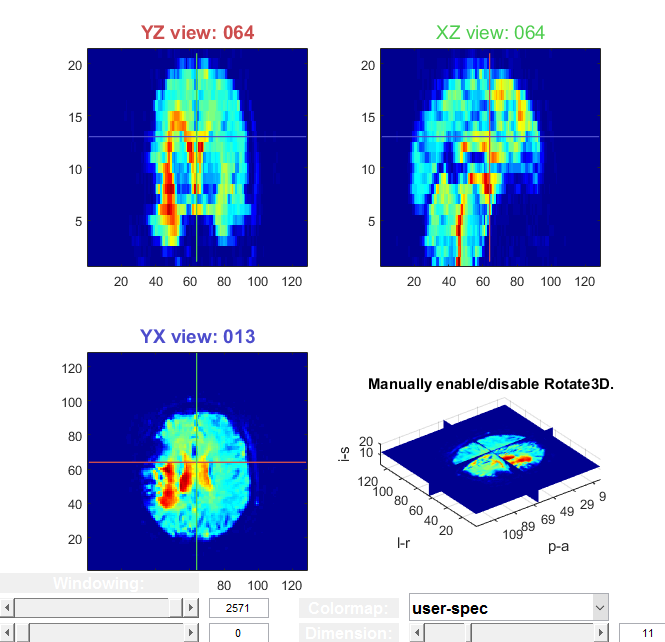
\includegraphics[scale=0.8,angle=0]{Images/4D.png}
    \caption{Programme Matlab pour la visualisation de données en 4D.}
    \label{fig:4D}
\end{figure}

\chapter{Choix automatique du nombre de classe.}

\section*{Algorithme 1 : Analyse des valeurs propres et le n-gap}

Dans le cas d'une classification idéale, la matrice laplacienne $L$ peut être mise sous la d'une matrice par bloc où tout les blocs non-diagonaux sont nuls.

\medskip

$
L = 
\begin{bmatrix}
   x^{(1)} &0 &\cdots &0 \\
   0 &x^{(2)} &\ddots &\vdots\\
   \vdots &\ddots &\ddots &0\\
   0 &\cdots &0 &x^{(n)}
\end{bmatrix}
$

\medskip

Cela traduit le fait que les blocs ou clusters sont homogènes et ne présentent pas de similitude entre eux. Cependant, vu comment la matrice L est construite, la valeur propre 0 va avoir une multiplicité égale au nombre de bloc.

\medskip

Une première méthode consiste donc à afficher les $n$ premières valeurs propres de L et de "compter" le nombre de fois que la valeur propre 0 apparait. Dans le cas des données simulées ci-dessous:

\medskip

\begin{figure}[H]
\centering
    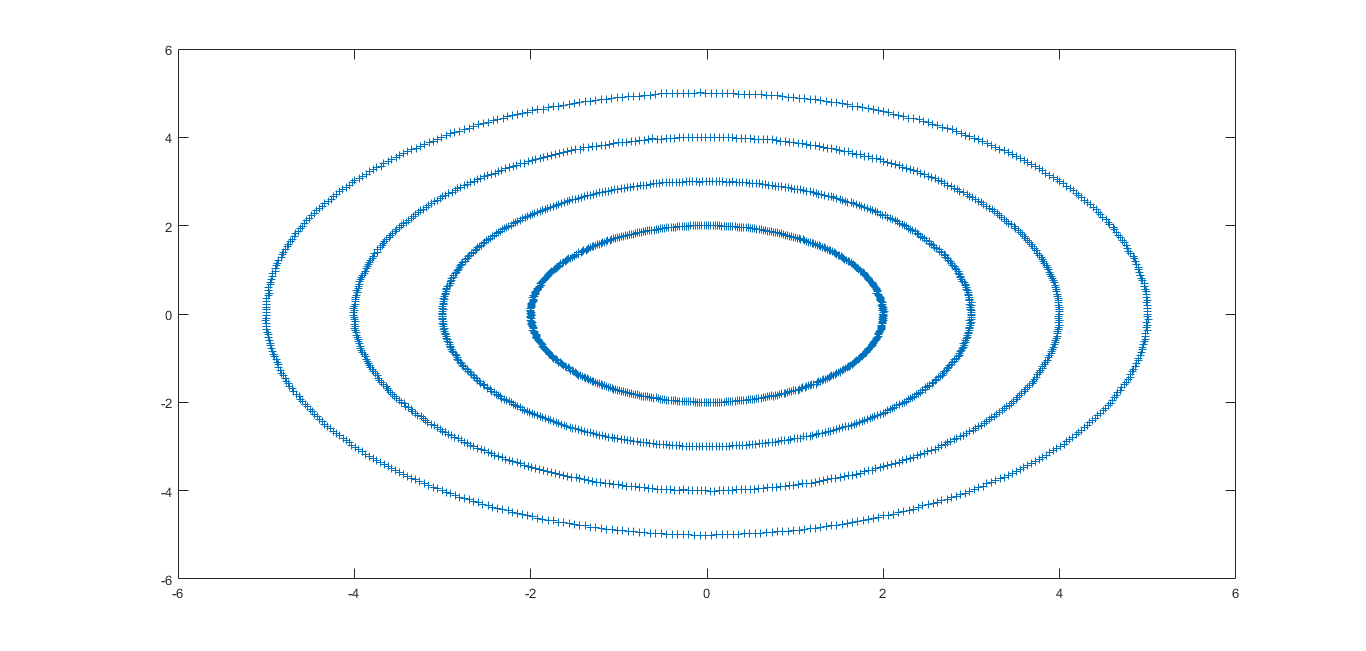
\includegraphics[scale=0.4,angle=0]{Images/testData.png}
    \caption{Exemple simple de données à classifier. Le nombre de classe est 4.}
    \label{fig:testData}
\end{figure} 

\medskip

Nous arrivons au valeurs propres suivantes:

\medskip

\begin{figure}[H]
\centering
    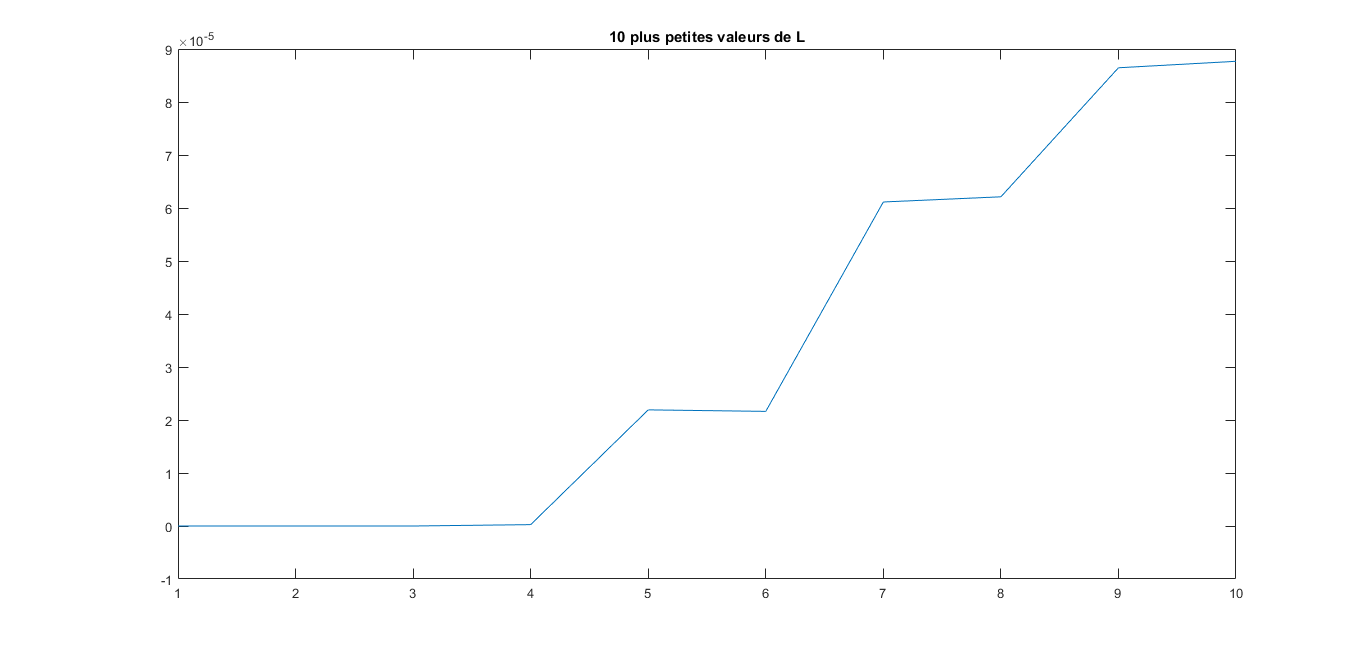
\includegraphics[scale=0.4,angle=0]{Images/Ngap.png}
    \caption{10 plus petites valeurs propres de L. On observe bien que on a un saut à partir de n=5. Le nombre optimal de classe est 4.}
    \label{fig:Ngap}
\end{figure} 

\medskip

Une autre méthode consiste à calculer la différence entre deux valeurs propres successives et voir à partir de quand un gap significatif se produit afin d'identifier le nombre de classe optimale. Néanmoins, ces deux méthodes sont hautement discutables de par leur manque de rigueur.


\section*{Algorithme 2 : Minimisation par la norme de Frobenius}

Une autre méthode consiste à voir pour quel nombre de classe la similitude entre classe est la plus faible.
On définit la norme de Frobenius d'une matrice par la formule suivante:

\medskip
$
\|{L}\|_F = \sum_{i=1}^{N_i}  \sum_{j=1}^{N_j} |L_{ij}|
$
\medskip

L'idée va donc être de calculer le volume des blocs diagonaux et de calculer une fonction coût qui dépend du nombre de classe.

\begin{figure}[H]
\centering
    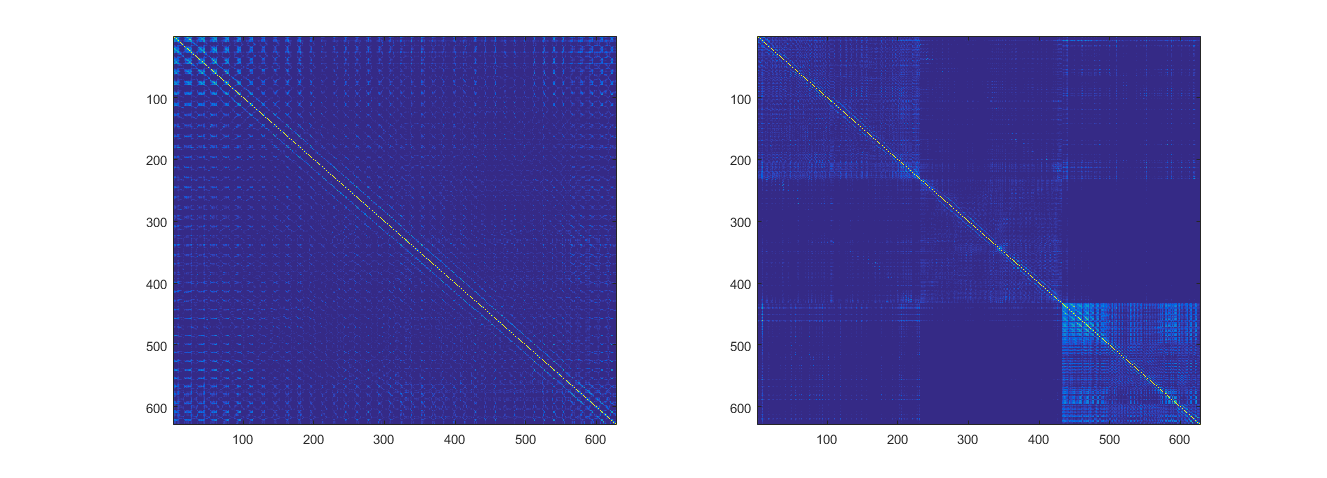
\includegraphics[scale=0.4,angle=0]{Images/L.png}
    \caption{Exemple de matrice laplacienne avant et après utilisation de l'algorithme de classification spectrale en trois classes et ré-agencement. On observe bien l'apparition de blocs.}
    \label{fig:L}
\end{figure} 

On définit donc le ratio de Frobenius entre deux blocs de la matrice L par:

\medskip

$
r_{ij} = \frac{ \|{L^{ij}}\|_F }{\| L^{ii} \|_F}
$

\medskip

On va donc regarder les valeurs de $r_{ij}$ et voir pour quel valeur de $n$ on atteint un minimum. Le but de cet algorithme va consister à trouver la valeur de $n$ qui va minimiser la fonction :

\medskip

$
\nu_k = \frac{2}{k(k-1)}\sum_{i=1 , j=i+1}^{k}(r_{ij})
$

\medskip

Il faut donc regarder pour plusieurs valeurs de n quel est le nombre de classe qui minimise cette fonction.

\section*{Application de ces algorithmes sur des données réelles.}

Sur des données simulées, les algorithmes précédents donnent de bons résultats mais cela n'est absolument pas le cas pour les données issues des IRM de cerveau. Les algorithmes ne semblent pas capables de déterminer de façon claire un nombre de classe optimal pour les signaux.

\chapter{Réalisation de programme pour le milieu médical en stand-alone.}

La société MathWorks propose un outil pour la réalisation de programme utilisant directement les fichiers Matlab. A partir d'une interface qui peut être très facilement crée par l'outil GUIDE de Matlab, on peut assez facilement proposer un programme qui peut être installé sur tout ordinateur ayant Windows comme système d'exploitation. 

\begin{figure}[H]
\centering
    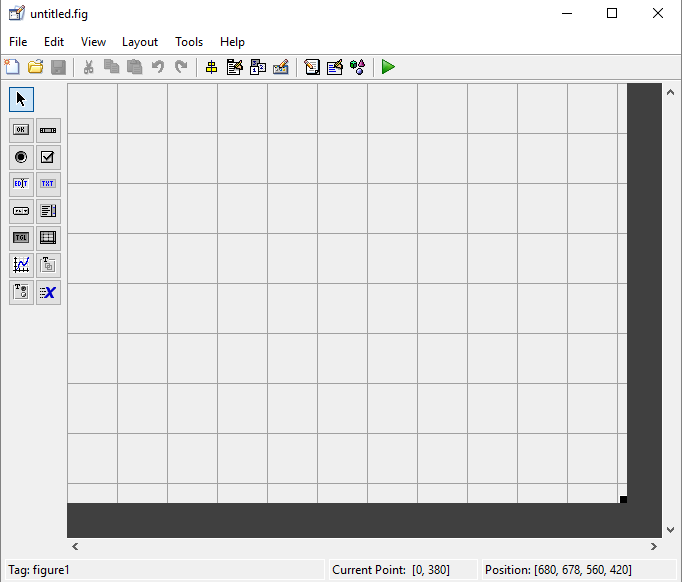
\includegraphics[scale=0.4,angle=0]{Images/Guide.png}
    \caption{Présentation de l'outil de Guide de Matlab.}
    \label{fig:Guide}
\end{figure} 

\begin{figure}[H]
\centering
    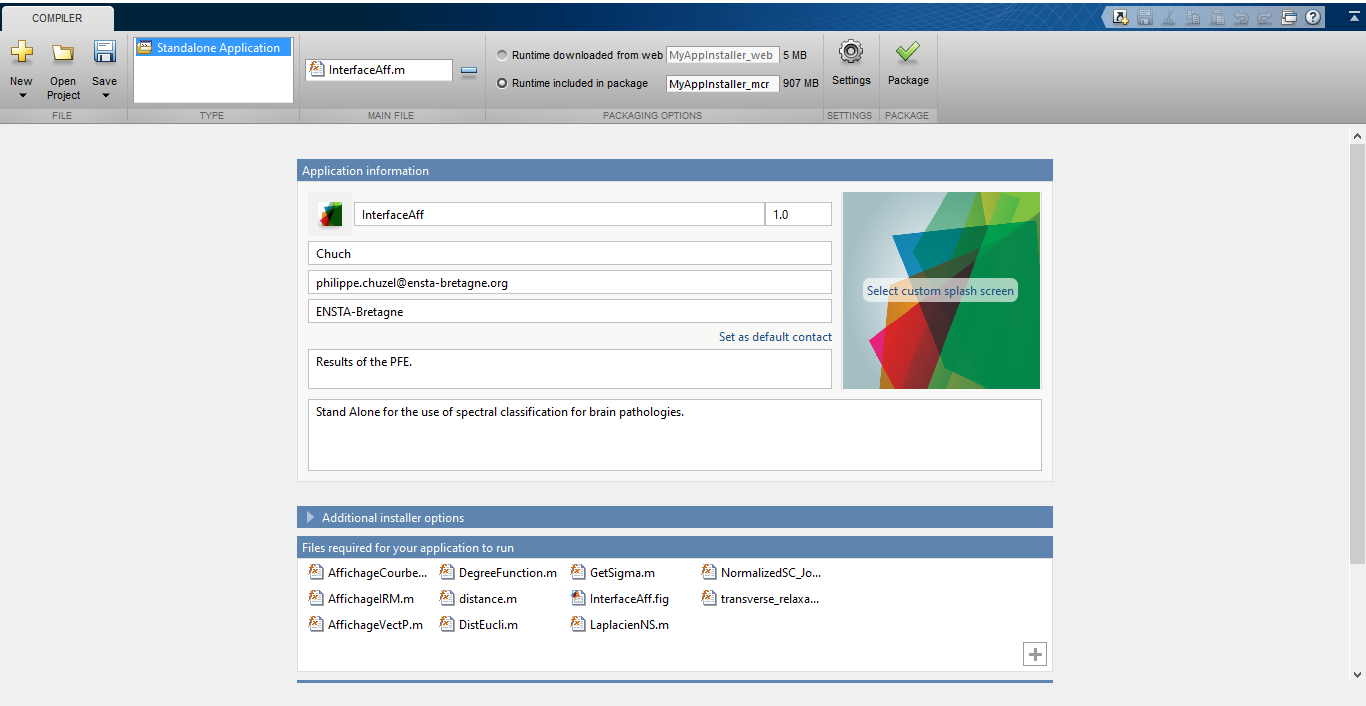
\includegraphics[scale=0.4,angle=0]{Images/StandAlone.png}
    \caption{Présentation de l'outil de Application Compiler de Matlab.}
    \label{fig:Compiler}
\end{figure} 

Néanmoins, l'exécutable qui est généré est très lourd, autour de 1GB ce qui est assez contraignant. Ce sont surtout les dépendance avec les bibliothèques en C et C++ qui impose un tel volume.

La meilleur solution si nous souhaitons avoir un programme entièrement portable est donc de passer le code en C++ et de réaliser une interface avec une bibliothèque adaptée du type QT.

\chapter{Rappel sur la théorie des graphes.}

\section{Définitions de base.}

Un graphe est constitué du couple (V,E,W), où V correspond à ensemble des nœuds du graphe, E correspond à l'ensemble des couple $(v_i,v_j)$ symbolisant le lien entre deux nœuds et W correspond à la matrice de voisinage. Par définition, le coefficient $W_{ij}$ prend comme valeur le poids liant le nœud $v_i$ au nœud $v_j$. Il s'en suit que la matrice W est symétrique. Nous verrons plus tard comment nous pouvons construire une tel matrice.


Par la suite, nous définissons la matrice D, diagonale, qui contient les degrés des nœuds du graphe. Le degré d'un nœud est défini par $d_i = \Sigma_{v_j \in V} W_{ij}$. 
\section{Choix du laplacien de la matrice.}

Il existe trois définition différentes de laplacien d'une matrice. Si on appelle $D$ la matrice de degré du graphe et $W$ la matrice de voisinage du graphe, on aboutie aux définitions suivantes.

\paragraph{Matrice Laplacienne standard non normalisée}

\medskip 

Ce laplacien est donné par la relation:

\begin{equation}
L = D-W
\end{equation}


\paragraph{Matrice Laplacienne normalisée asymétrique}

\medskip 

Ce laplacien est donné par la relation:

\begin{equation}
L = I-D^{-1}W
\end{equation}


\paragraph{Matrice Laplacienne normalisée symétrique}

\medskip 

Ce laplacien est donné par la relation:

\begin{equation}
L = I-D^{-1/2}WD^{-1/2}
\end{equation}

Ces trois matrices présentent les mêmes propriétés:

\begin{itemize}
\item Ces matrices présentent la valeur propres 0 une seule fois pour le vecteur propre $I$ ou $D^{1/2}I$.
\item Ces matrices sont réelles semi-définies positives.
\end{itemize}

Par conséquent, quand nous chercherons à trouver les k plus petites valeurs propres de cette matrice, il nous sera possible très facilement de les récupérer.

\chapter{Construction de la matrice de voisinage.}


Il y a trois choix à faire pour définir la matrice de voisinage d'un graphe.

\section{Choix du type de voisinage.}

Pour un ensemble de nœud donné, il y a plusieurs manière de créer les liens qui vont compléter l'ensemble (E,V,W).

\medskip

\textbf{Graphe des epsilons voisin}: On considère ici que deux nœuds ont un lien si la distance entre eux est inférieur à $\epsilon$.

\medskip

\textbf{Graphe des k-plus proche voisins}: On considère ici que tous les nœuds ont k voisins et qu'ils sont les k-plus proche du nœud considéré.

\medskip

\textbf{Graphe entièrement connecté}: On considère que tous les sommets sont reliés entre eux. 

\medskip

Ici, nous avons implémenté le graphe entièrement connecté car il nous donne de très bons résultats et qu'il est très simple à mettre en place.

\section{Choix de la distance et de la similitude.}

Dans la littérature de la classification, il est nécessaire de choisir une distance et une fonction de similarité.

\medskip

Plusieurs choix s'offre à nous pour les distances:

\begin{itemize}

\medskip

\item \textbf{Distance de Manhattan} : $\Sigma_i|x_i-y_i|$

\medskip

\item \textbf{Distance d'euclidienne} : $(\Sigma_i(x_i-y_i)^2)^(1/2)$

\medskip

\item \textbf{Distance de Minkowski} : $(\Sigma_i|x_i-y_i|^p)^(1/p)$

\medskip

\end{itemize}

La distance euclidienne a ici été choisie.

\medskip

La fonction de similitude doit être une fonction qui va associer une valeur comprise entre 0 et 1 à deux sommet du graphe:

\begin{equation}
f(x_i,x_j) \Rightarrow [0 ; 1]
\end{equation}

La littérature donne plusieurs types de fonction de similitude mais deux sont à retenir.
\begin{itemize}

\item La similitude euclidienne qui est définie par la fonction \\
\begin{equation}
f(x_i,x_j) = \frac{1}{1+\frac{d^2(x_i,x_j)}{\sigma^2}}
\end{equation}

\item La similitude gaussienne qui est définie par la fonction \\
\begin{equation}
f(x_i,x_j) = exp(-\frac{d^2(x_i,x_j)}{2\sigma^2})
\end{equation}

\end{itemize}


Dans les deux cas, le coefficient $\sigma$ est un paramètre qui traduit la dispersion des données. Nous avons ici choisi la similitude gaussienne car elle permet de traduire de manière plus efficace la similitude des données.
 
\section{Choix du paramètre de dispersion.}

Le gros problème pour les données que nous aurons à traiter est que le paramètre $\sigma$ devra être déterminé de manière automatique en fonction des données d'entrées.Ce paramètre va traduire la similitude ou non des différents éléments entre eux et donc va conditionner tous les résultats de l'algorithme.

\medskip

Pour ce faire, une solution assez élégante a été proposée \cite{zelnik2004self} et consiste à définir le paramètre $\sigma$ comme le produit $\sigma_i\sigma_j$, où ces deux coefficient dépendent du voisinage de chaque point.

\medskip

Ainsi, on définit le coefficient par $\sigma_i = d(x_i,x_r)$ où $x_r$ correspond au r-ième voisin le pus proche de $x_i$. Après beaucoup de test, on constate comme dans le document \cite{tartare2014contribution} que les meilleurs résultats sont obtenus pour $r=7$ ou $r=9$.




\chapter{Quels algorithmes de classification spectrale?}


Les algorithmes de classification spectrale sont répartis en deux classes:

\begin{itemize}
\item La première classe qui va faire une séparation en deux groupes de manière récursive à partir de la seconde plus petite valeur propre de la matrice laplacienne issue du graphe jusqu'à avoir k clusters.
\item La seconde consiste à faire une classification sur les k plus petits vecteurs propres de la matrice laplacienne issue du graphe grâce à un algorithme plus simple comme le K-means.
\end{itemize}

\medskip


Dans le cadre de ce projet, nous avons principalement étudié la seconde classe d'algorithme de classification et particulièrement celui développé par Jordan and Weiss. Au total, nous avons implémenté 4 algorithmes différents de classification spectrale. Les détails théoriques de ces algorithmes peuvent être trouver dans ces références \cite{von2007tutorial} et \cite{shi2000normalized}.

\medskip

Les trois premiers algorithmes correspondent à la seconde classe d'algorithme alors que le dernier algorithme appartient à la première classe d'algorithme:

\begin{algorithm}[H]
  \caption{Unnormalized spectral clustering }
  
  \textbf{Entrées}% Inputs section
  \begin{algorithmic}[1]
    \STATE Matrice $W$ matrice de voisinage
    \STATE Entier $k$ nombre de classe
  \end{algorithmic}
  \bigskip

  \textbf{Sorties}% Output section
  \begin{algorithmic}[1]
    \STATE Vecteur $Ver$ table de vérité calculée.
  \end{algorithmic}
  \bigskip
  
  \textbf{Algorithme}
  \begin{algorithmic}[1]
		\STATE $L\gets$ Laplacien standard de la matrice $W$
     	\STATE $VectP\gets$ matrice contenant les vecteurs propres des k plus petites valeurs propres non nulles de L
     	\STATE $Ver\gets$ résultat de l'algorithme du Kmeans sur la matrice VectP en k clusters.	
  \RETURN $Ver$
  \end{algorithmic}
\end{algorithm}



\begin{algorithm}[H]
  \caption{Normalized spectral clustering, Shi and Malik }
  
  \textbf{Entrées}% Inputs section
  \begin{algorithmic}[1]
    \STATE Matrice $W$ matrice de voisinage
    \STATE Entier $k$ nombre de classe
  \end{algorithmic}
  \bigskip

  \textbf{Sorties}% Output section
  \begin{algorithmic}[1]
    \STATE Vecteur $Ver$ table de vérité calculée.
  \end{algorithmic}
  \bigskip
  
  \textbf{Algorithme}
  \begin{algorithmic}[1]
		\STATE $L\gets$ Laplacien asymétrique de la matrice $W$
     	\STATE $VectP\gets$ matrice contenant les vecteurs propres des k plus petites valeurs propres non nulles de L
     	\STATE $Ver\gets$ résultat de l'algorithme du Kmeans sur la matrice VectP en k clusters.	
  \RETURN $Ver$
  \end{algorithmic}
\end{algorithm}




\begin{algorithm}[H]
  \caption{Normalized spectral clustering, Jordan and Weiss }
  
  \textbf{Entrées}% Inputs section
  \begin{algorithmic}[1]
    \STATE Matrice $W$ matrice de voisinage
    \STATE Entier $k$ nombre de classe
  \end{algorithmic}
  \bigskip

  \textbf{Sorties}% Output section
  \begin{algorithmic}[1]
    \STATE Vecteur $Ver$ table de vérité calculée.
  \end{algorithmic}
  \bigskip
  
  \textbf{Algorithme}
  \begin{algorithmic}[1]
		\STATE $L\gets$ Laplacien symétrique de la matrice $W$
     	\STATE $VectP\gets$ matrice contenant les vecteurs propres des k plus petites valeurs propres non nulles de L
     	\STATE normaliser toutes les lignes de la matrice $VectP$
     	\STATE $Ver\gets$ résultat de l'algorithme du Kmeans sur la matrice VectP en k clusters.	
  \RETURN $Ver$
  \end{algorithmic}
\end{algorithm}

\medskip



\medskip

\begin{algorithm}[H]
  \caption{Normalized spectral recursive clustering, Shi and Malik }
  
  \textbf{Entrées}% Inputs section
  \begin{algorithmic}[1]
    \STATE Matrice $W$ matrice de voisinage
    \STATE Entier $k$ nombre de classe
  \end{algorithmic}
  \bigskip

  \textbf{Sorties}% Output section
  \begin{algorithmic}[1]
    \STATE Vecteur $Ver$ table de vérité calculée.
  \end{algorithmic}
  \bigskip
  
  \textbf{Algorithme}
  \begin{algorithmic}[1]
		\STATE $L\gets$ Laplacien asymétrique de la matrice $W$
     	\STATE $VectP\gets$ seconde plus petite valeur propre de L
     	\STATE Partititionner le graphe en deux sous-ensemble selon les valeurs de $VectP$
     	\STATE Répéter l'algorithme jusqu'à avoir k clusters.
     	\STATE $Ver\gets$ résultat de l'algorithme.	
  \RETURN $Ver$
  \end{algorithmic}
\end{algorithm}

